\subsection{Design}
I denne sektion er beskrevet hvorledes klienten er opbygget. Klienten står for at modtage besked objekter fra applikations laget, og omsætte disse til strings der kan sendes til serveren. Desuden står klienten for at modtage svar fra serveren, og omdanne disse til den korrekte beskedtype. Klientens opbygning er vist i UML diagram på figur~\ref{fig:ConnectionClient}
\begin{figure}
	\centering
	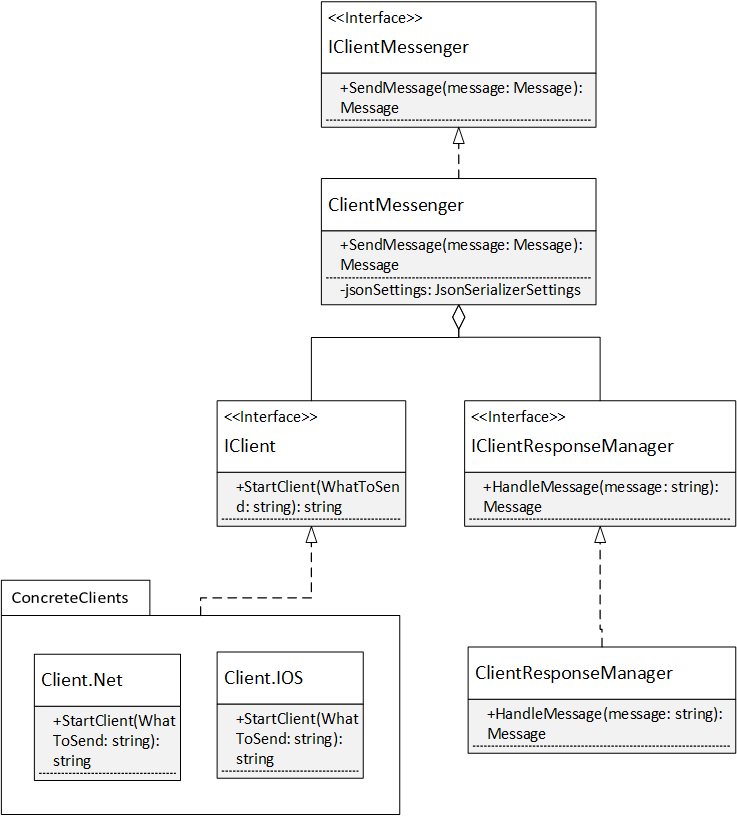
\includegraphics[width=0.9\linewidth]{figs/connection/ConnectionClient.png}
	\caption{Klient diagram}
	\label{fig:ConnectionClient}
\end{figure}

Et eksempel på et typisk forløb i klienten er vist på figur~\ref{fig:ClientSequence}
\begin{figure}
	\centering
	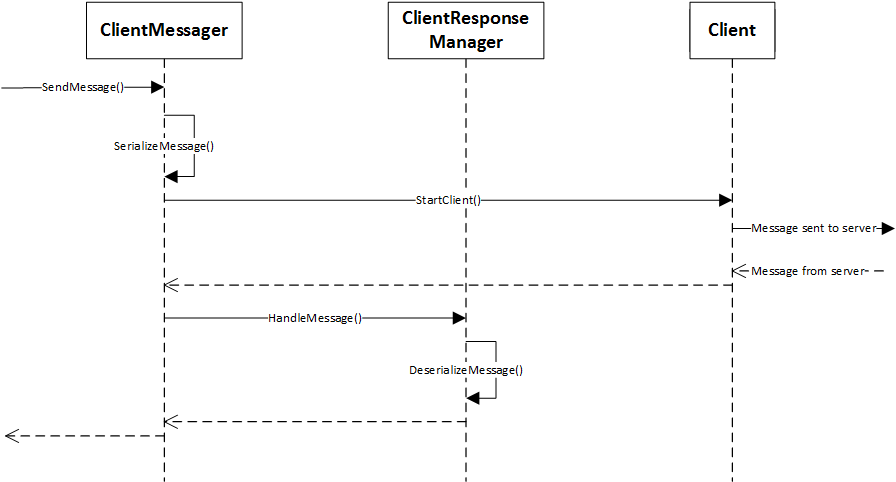
\includegraphics[width=0.9\linewidth]{figs/connection/ClientSequence.png}
	\caption{Client Sequence Diagram}
	\label{fig:ClientSequence}
\end{figure}

\subsection{Implementering}
I denne sektion er beskrevet hvordan de enkelte komponenter, der tilsammen udgør klienten, er realiseret.

\subsubsection{Synchronous Socket Client}
Er den konkrete implementering af socket client, som anvendes med en windows desktop applikation. Klassen er implementeret udfra eksemplet fundet på https://msdn.microsoft.com/en-us/library/kb5kfec7(v=vs.110).aspx ?? . Der er tilføjet exception handling, i tilfælde af at serveren ikke svarer. Andre konkrete klienter er baseret på samme princip.

\subsubsection{ClientMessenger}
Modtager et besked objekt fra applikations laget. Dette bliver serializeret til en string vha. Json. Der anvendes JsonSettings da det er nedarvede objekter som serializeres, og der derfor er behov for flere oplysninger om objektet, end hvad der som standard genereres med Json. Derefter sendes beskeden vha. en IClient og en IClientReponseManager håndterer svaret før det returneres til applikations laget. Dette ses af koden i listing~\ref{code:ClientSendMessage} 
\begin{lstlisting}[caption=Client.SendMessage,label=code:ClientSendMessage]
public Message SendMessage(Message message)
{
	return _clientResponseManager.HandleMessage(_client.StartClient(JsonConvert.SerializeObject(message, _jsonSettings) + "<EOF>"));
}
\end{lstlisting}

\subsubsection{Client Response Manager}
Modtager en string som indeholder informationer om et objekt. Ved først at deserializere objektet til basis klassen message, oprettes en switch case på beskedens type som vist på listing~\ref{code:ClientHandleMessage}
\begin{lstlisting}[caption=Client.HandleMessage,label=code:ClientHandleMessage]
public Message HandleMessage(string messageString)
{
	var receivedMessage = JsonConvert.DeserializeObject<Message>(messageString);
	
	switch (receivedMessage.MsgType)
	{
		case MessageTypes.LoginResponse:
		return JsonConvert.DeserializeObject<LoginResponseMsg>(messageString);
		
		case MessageTypes.GeneralResponse:
		return JsonConvert.DeserializeObject<GeneralResponseMsg>(messageString);
		
		case MessageTypes.GetPoolDataResponse:
		return JsonConvert.DeserializeObject<GetPoolDataResponseMsg>(messageString);
		
		case MessageTypes.GetPoolInfoResponse:
		return JsonConvert.DeserializeObject<GetPoolInfoResponseMsg>(messageString);
		
		default:
		if (receivedMessage.MessageInfo != null)
			return new Message(receivedMessage.MessageInfo);
		else
		{
			return new Message("An unknown error occured");
		}
	}
}
\end{lstlisting}